\chapter{基于RDMA的Plasma数据传输机制实现}

在本章节中,我们将基于上一章对Plasma架构和性能的分析,提出并实现一种适应各大小数据的高吞吐数据传输机制。由于跨节点通信完全由Manager进程完成,因此在本章节中,
如无特殊说明,进程均指的是Manager进程。

\section{连接的建立和复用}

要进行双边(Send/Recv)和单边(Read/Write)通信,通信两端都需要首先为建立Infiniband连接。和套接字简单的连接过程不同,在双方能够通过发送事务传送数据之前,首先要完成
如下准备工作:

\begin{enumerate}
	\item 创建IB上下文(Context);得到机器的IB设备列表,并打开其中一个设备(网卡)。用户可以在此时读取网卡的部分硬件参数。
	\item 创建一个保护域(Protection Domain,PD)。这是一种管理机制,后续创建的数据结构只有处在同一个保护域中才能相互访问。
	\item 创建发送/接收缓冲区,并将其注册为内存区域(Memory Region,MR)。这一操作的主要目的是使内存页面驻留在物理内存中,防止操作系统通过换页等机制
	将内存空间移出。由于RDMA实现在用户态,缓冲区的检查和数据收发都需要由用户正确地管理——否则会导致旧数据被覆盖等错误。
	\item 创建完成队列(Completion Queue,CQ)。在双边通信中,用户通过拉取完成队列来检查通信事务的执行结果。
	\item 双方进程创建并连接队列对(Queue Pair,QP)。使用可靠连接(RC)服务时,一对队列对在建立连接后只能相互发送数据。要建立一对连接,
	用户需要使用套接字等基础通信手段交换队列对的关键参数:网卡设备的本地编号(lid)和队列对编号(qp\_num)。
\end{enumerate}

IB连接的建立流程有显著的时间开销。在实验中,我们通过测试发现这一流程将引入额外300ms左右的延迟开销。这一结果和\cite{}的描述基本一致。尽管由于面向单机,这一开销
在高并发内存系统的相关研究中并没有得到很大重视,然而这对于分布式内存系统Plasma来说是重要的。后者在每个节点都要部署进程,其IB连接以$O(N^2)$速度扩大规模。
加之Plasma具有不规律的通信特征,即便是基于套接字的实现,大量并发的连接请求也造成了显著的性能损失。因此在集群中反复建立IB连接更是难以忍受的。

所以,我们必须在节点间复用IB连接。值得注意的是,步骤3创建并固定内存缓冲区占用了上述过程的主要时间开销,并且这一过程不依赖于队列对的连接。所以,在IB优化的Plasma
实现中,我们先尝试建立队列对,然后才分配缓冲区。我们为每个进程维护了一个以网卡编号lid为键的哈希表。哈希表中的每个元素,以一个数据结构保存着一对IB连接的必要数据。因此,当两个进程尝试建立连接时,
它们将首先通过套接字交换lid,并查找哈希表。如果两个节点曾经建立过IB连接,那么双方将复用第一次分配好的缓冲区。通过这一改进,Plasma仅有初次IB连接会感受到明显的传输延迟,而重复连接的时间开销大幅降低。

\section{基于双边通信的传输协议}

针对内存数据库常见的较小数据,我们提出了基于双边通信机制的传输协议。这一机制的优势在于,能够充分利用两节点间预先分配的发送/接收缓冲区。其示意图如\autoref{fig:send_protocol}所示:

\begin{figure}[h]
	\centering
	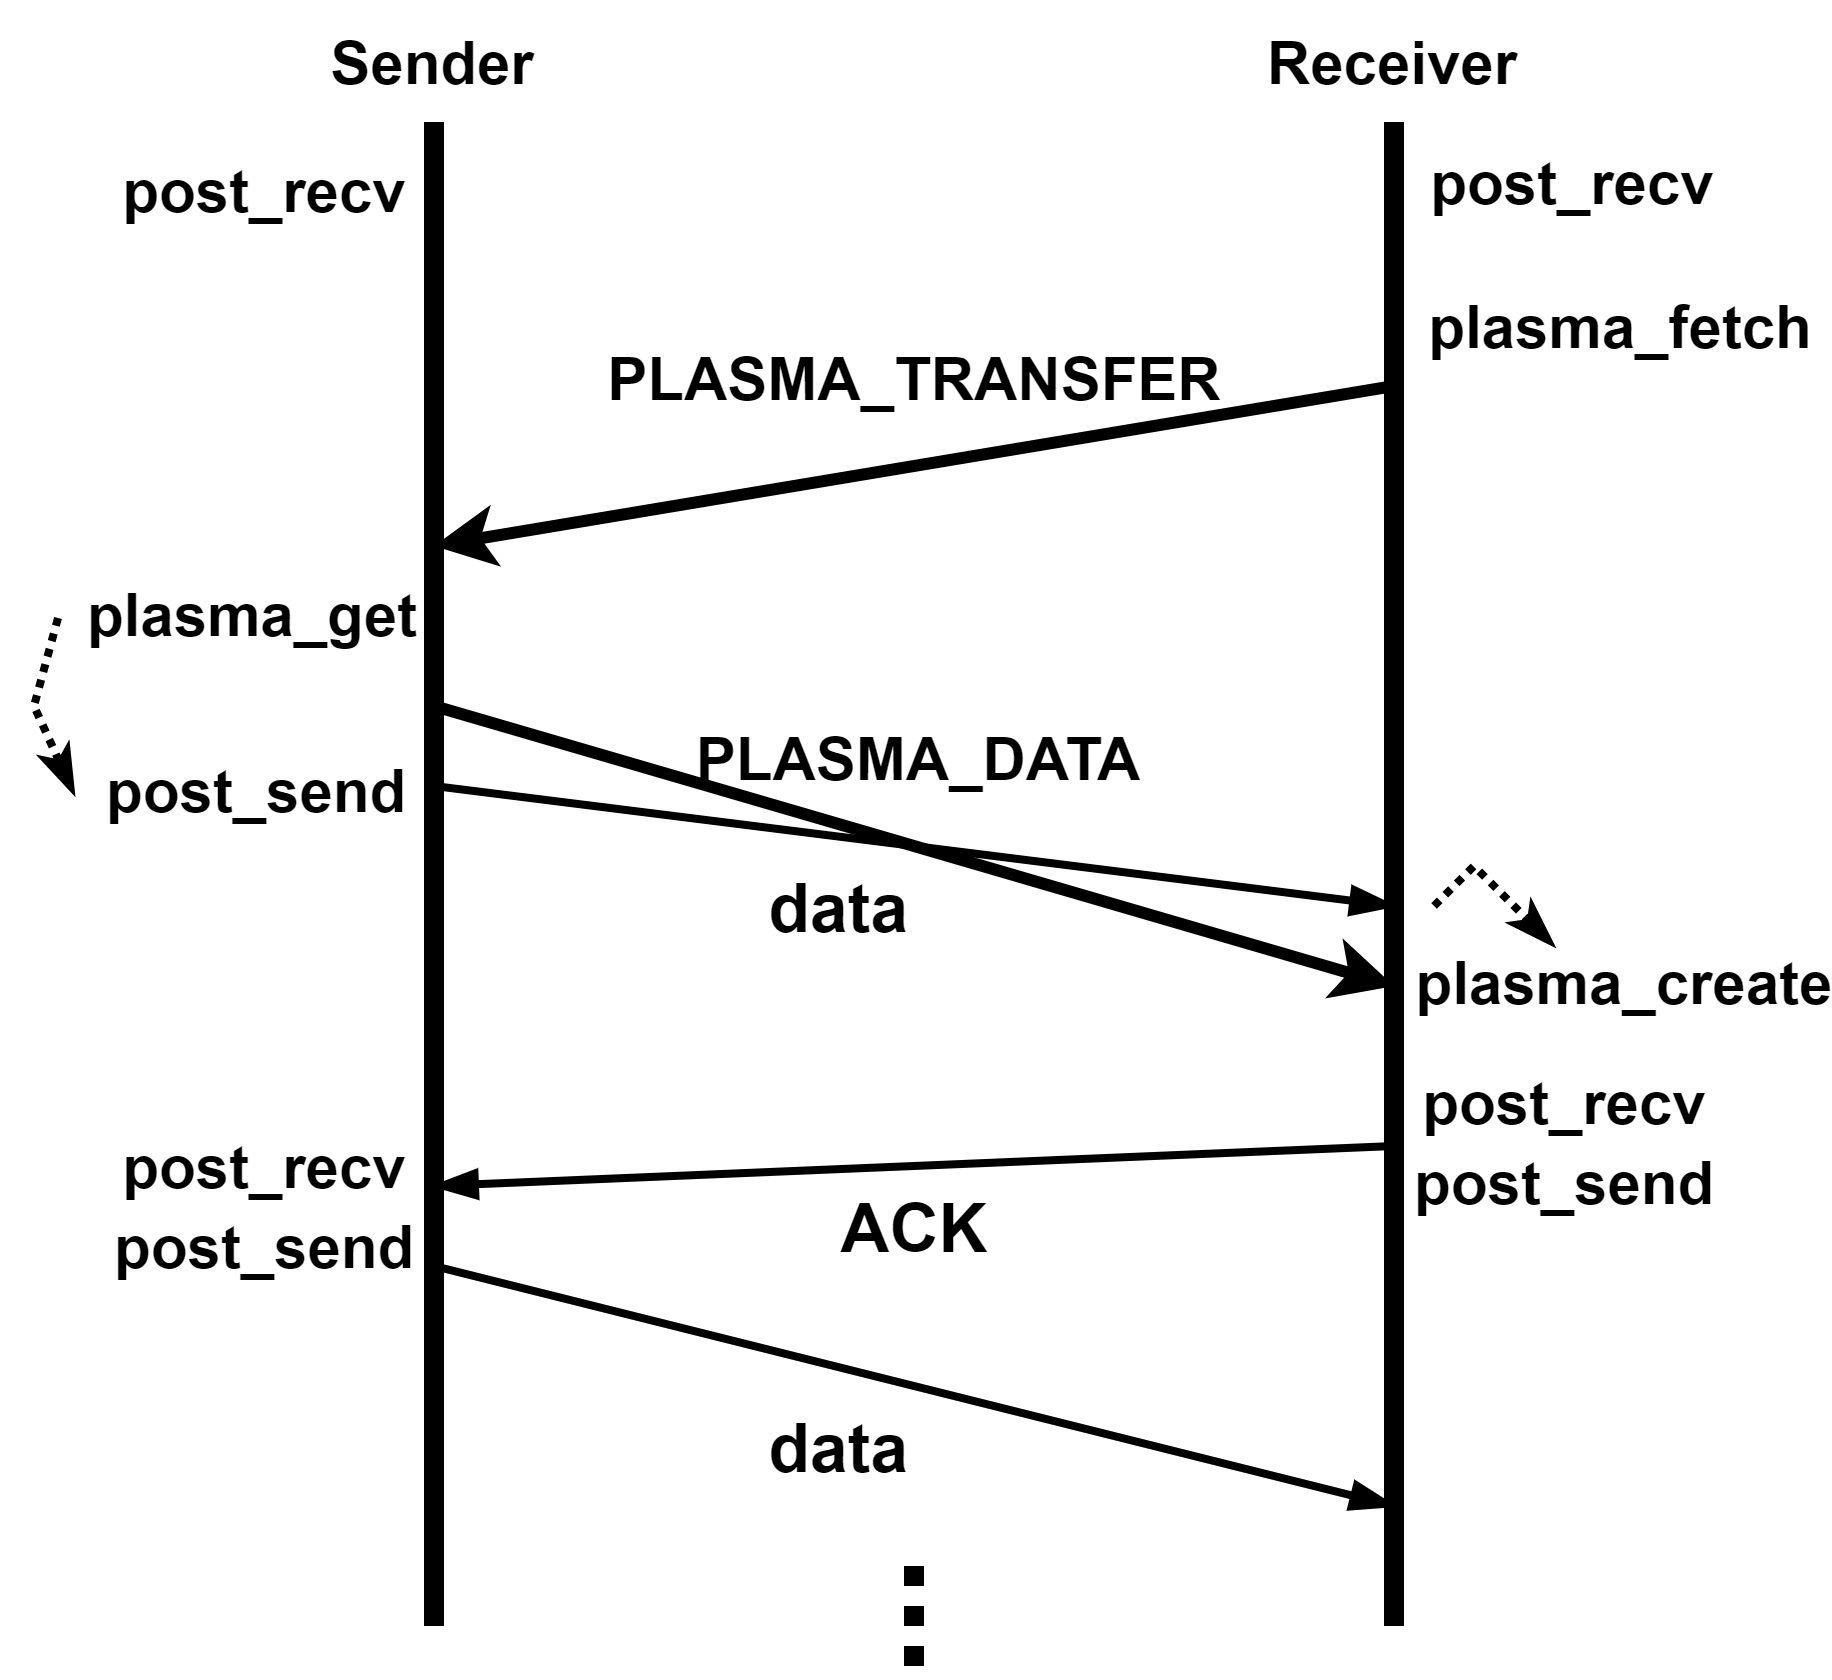
\includegraphics[width=0.7\textwidth]{image/chap03/send_protocol.png}
	\caption{基于双边通信的传输协议}
	\label{fig:send_protocol}
\end{figure}

在该传输协议中,通信双方(Sender/Receiver)在握手发生前必须首先通过一次post\_recv操作将一个接收事务放入到接收队列中。这是因为任何一个发送事务在完成时,连接的接收队列必须有可用的接收事务对应,
否则通信无法发生。在本实现中,由于每个进程都维护着与其他进程的IB连接和对应的缓冲区,因此做法是在连接建立时,进程都首先将一个接收事务放入到和该连接关联的接收队列中。这样我们就能确保第一次数据传输的
握手发生前,接收队列总是存在可用的接收事务。

当数据发送方收到类型为PLASMA\_TRANSFER的消息后,和套接字协议一样,它首先调用plasma\_get函数得到了数据缓冲区的地址。然后,发送方将对象id、数据大小等关键元数据通过PLASMA\_DATA消息传递给数据接收方。
之后,发送方将数据从得到的内存拷贝到预留的发送缓冲区,调用post\_send将数据通过RDMA发送到接收方预留的接收缓冲区。值得注意的是:

\begin{enumerate}
	\item 以此协议发送和接收数据,发送方和接收方在这一阶段都会产生一次用户态的内存拷贝。如\autoref{fig:send_protocol}中虚线箭头所示:为了复用预先分配的内存缓冲区、避免重复的内存分配和注册,
	发送前数据必须要拷贝到固定缓冲区,接收时必须要从固定缓冲区拷贝。在较小数据的传输中,这两次内存拷贝的开销占比较低,因而是较优的通信方案。
	\item RDMA传输的数据和接收方调用plasma\_create的顺序是不定的,但不影响该协议的正确性,\autoref{fig:send_protocol}展示了其中一种顺序。数据可能先于元数据到达,也可能后于元数据到达。但不论事件以何种顺序发生,
	接收方都会在元数据到达后,调用plasma\_create创建对象,然后轮询完成队列(CQ),确保对象数据已经到达。最后通过一次用户态的内存拷贝,将数据存到指定位置。在这里,轮询完成队列充当了同步的角色——如果数据已经到达,
	它将立刻返回;否则将阻塞,直到数据在缓冲区准备就绪。这一现象展示了RDMA通信的异步性。
\end{enumerate}

\textbf{接受事务的补充}:数据到达后,由于接收事务被消耗了,接收方在取出数据、确认缓冲区可覆盖之后,需要重新提交一个接受事务等待下次使用。
在这一步,我们希望从完成队列里面获取接收数据的内存地址,以便将一个指向相同地址的接收事务补充到接收队列中。这一目的可以通过事务编号(Work Request ID)完成:IB的事务编号是一个64位无符号整数,因此我们可以直接将接收地址
作为事务的编号——这样还很方便地解决了事务编号的唯一性。

\textbf{发送确认信息:}和基于套接字的协议不同,此时接收方还需要发送一个确认(ACK)消息给发送方。因为发送方并不知道接收方何时重新准备好了
接收事务和缓冲区(而这在套接字编程中是无需担心的),这一ACK消息用于启动下一轮的数据发送。如果没有这一确认消息,发送方可能会在接收方没有配对的接收事务时再次发送,进而导致程序错误。

\section{基于单边通信的传输协议}

\textbf{双边协议的局限性:}在实现了上述基于双边通信的传输协议后,在实验中我们已经观察到了相当的吞吐提升——即便完成传输所需的通信次数相比套接字协议更多,但RDMA通信的延迟极低。然而,进一步对程序在较大数据的传输测试中进行性能采集,我们发现当数据规模增加时,程序将大量CPU时间
用于用户态的数据拷贝(即memcpy调用)。虽然,用户态的内存拷贝性能很高,在数据较小时导致的额外延迟并不显著,但随着数据增长到1M大小,CPU的处理能力无法跟上RDMA网卡的吞吐能力,成为了性能瓶颈。

对于上述双边通信的传输协议,选择用数据拷贝代替反复创建/销毁缓冲区是出于对后者较大开销的忌惮。这一前提在大型数据下是否还成立呢?结论是否定的,在第四章的实验和分析中,我们确认了内存空间分配+注册具有更好的扩展性:在数据较大时,
反而是CPU直接复制同样大小的数据更耗费时间。这一观察驱使我们进一步为较大数据单独设计一个支持零拷贝的传输协议。我们实现了基于单边读(One-sided Read)的约会(Rendezvous)协议,其示意图如\autoref{fig:read_protocol}所示:

\begin{figure}[h]
	\centering
	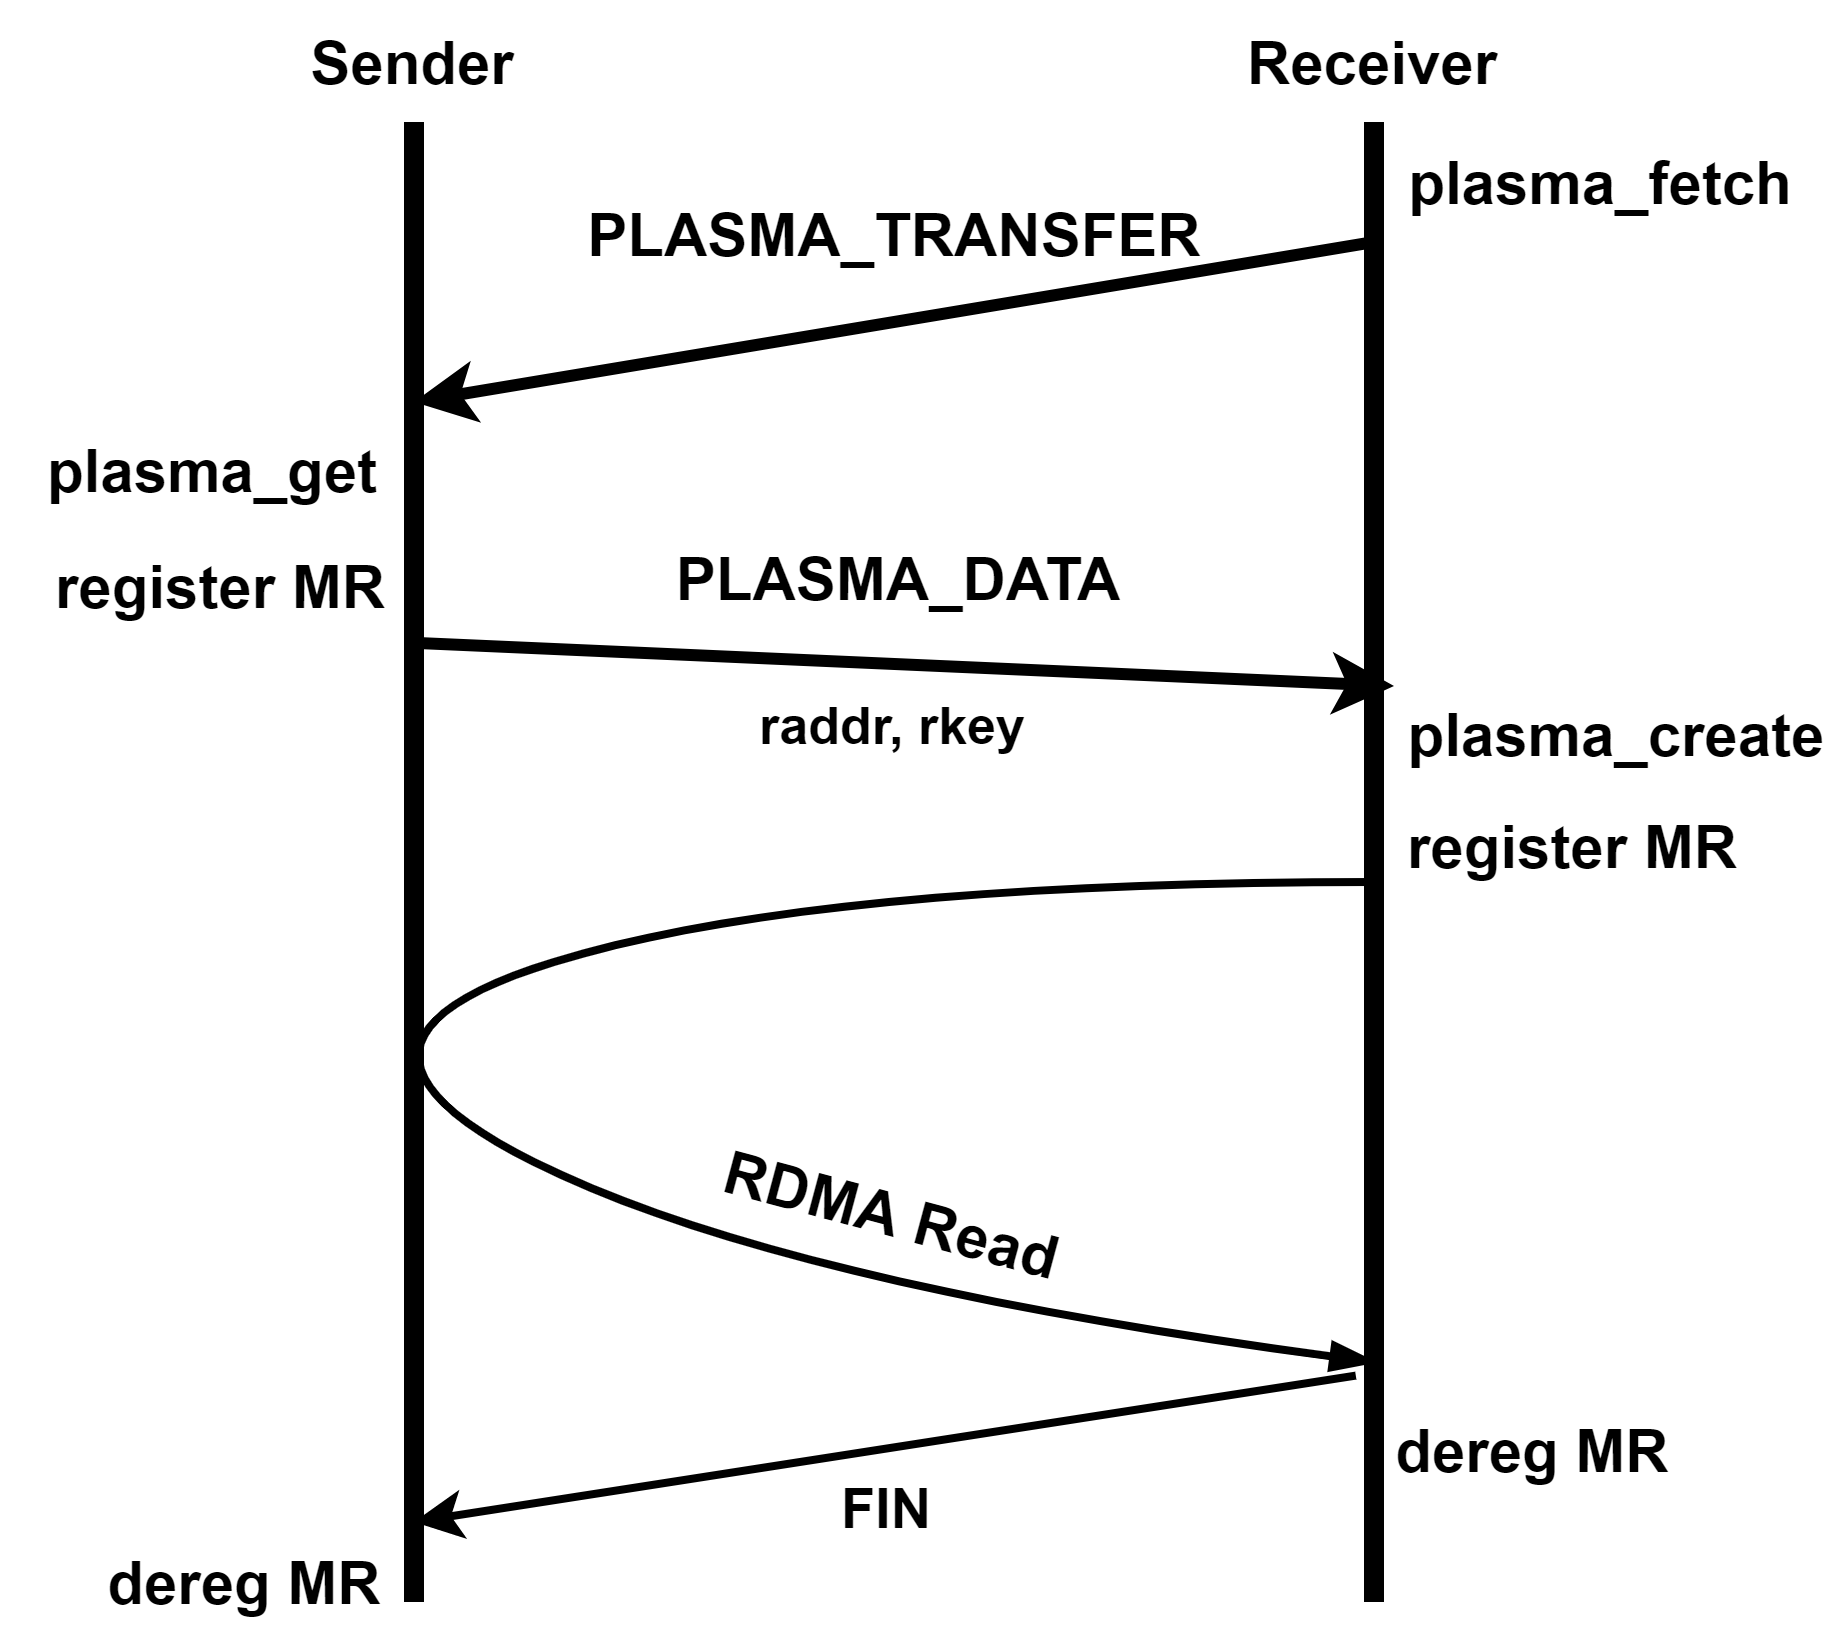
\includegraphics[width=0.7\textwidth]{image/chap03/read_protocol.png}
	\caption{基于单边通信的传输协议}
	\label{fig:read_protocol}
\end{figure}

在基于单边读的传输协议中,使用了与传统通信原语极为不同的读语义:发送方不再事实上承担发送数据的任务,而是由接收方直接从远端内存拉取数据到本地。在接受到PLASMA\_TRANSFER消息,且通过plasma\_get函数调用获得了数据对象的地址后,
发送方直接向RDMA网卡注册MMAP映射返回的内存空间。因此,内存数据将在原地被网卡读取并发送,而不再依靠预先分配的固定缓冲区。接下来,接收方将会收到发送方传递的元数据、创建内存空间,并同样向RDMA网卡注册plasma\_create返回的内存地址。
需要注意的是,这一阶段发送方需要额外地将本地内存地址(raddr, rkey)发送到接收方处,才能正确地引导后者拉取内存数据。
此时,双方的内存空间都已原地(in-place)成为可用的发送/接收缓冲区,接收方发出一个单边读请求,就能完成对象的复制。最后,接收方通过一个结束(FIN)消息通知对方注销缓冲区,也同时注销自己的缓冲区。一次数据传输就完成了。

\textbf{单边协议的技术优势:}在这一协议中,我们将内存数据所处空间原地注册为缓冲区,这一协议具有一些优势:传输仅需要两个来回(一次握手和一次传输),相比之下双边协议的来回数依赖于固定缓冲区的大小;实现比前者更简单;为发送方和接收方各节省了一次用户态的数据拷贝,
实验表明这一特性在数据较大时具有明显性能优势。

\section{混合传输机制实现}

上述的两种传输协议具有不同的性能表现,本质上是在两种固定开销中进行权衡:双边传输协议使双方增加了一次内存拷贝,避免了重复的内存注册/注销操作;单边传输协议每次传输都需要注册/注销内存,但真正实现了(用户态/内核态)内存零拷贝。直观上来说,
前者适合发送小数据,而大型数据则应该采用后者传输。幸运的是,通过确定一个分界点,我们能将两种机制混合实现,而只需要对Plasma主逻辑做出微小改动。定义常量IB\_READ\_MIN\_SIZE为采用单边协议的最小数据量,就能在函数调用前确定使用的协议。
下面伪代码展示了发送端和接收端的处理逻辑:

\begin{algorithm}[h]
	\caption{服务端发送机制}\label{server}
	\KwIn{连接上下文$conn$,对象标识符$id$}
	$buf$:缓冲区,$S_d$:数据大小,$S_m$:元数据大小 \\
	读取对象内存区域:$buf, S_d, S_m \leftarrow$ plasma\_get($id$) \\
	发送元数据:send\_message($conn, S_d, S_m, id$) \\
	\eIf{$S_d$ + $S_m$ $\leq$ IB\_READ\_MIN\_SIZE}{
		发送本地地址:ib\_send\_read\_info($conn, buf$) \\
		等待单边读:ib\_wait\_object($conn, buf$)
	}{
		双边发送协议:ib\_send\_object\_chunk($conn, buf$)
	}
	释放对象:plasma\_release($id$)
\end{algorithm}

\begin{algorithm}[h]
	\caption{客户端接收机制}\label{client}
	\KwIn{连接上下文$conn$}
	$buf$:缓冲区,$S_d$:数据,$S_m$:元数据大小,$id$:对象标识符 \\
	接收元数据:$S_d, S_m, id \leftarrow$ recv\_message($conn$) \\
	创建对象内存区域:$buf \leftarrow$ plasma\_create($id, S_d, S_m$) \\
	\eIf{$S_d$ + $S_m$ $\leq$ IB\_READ\_MIN\_SIZE}{
		$raddr$:远端内存地址 \\
		接收远程地址:$raddr \leftarrow$ ib\_recv\_read\_info($conn$) \\
		单边读协议:ib\_read\_object($conn, buf, raddr$)
	}{
		双边接收协议:ib\_recv\_object\_chunk($conn, buf$)
	}
	确认对象:plasma\_seal($id$) \\
	释放对象:plasma\_release($id$) \\
\end{algorithm}

在之后的实验中,我们将对套接字协议、双边传输协议和单边传输协议分别进行详细的性能测试,确定出最优的参数,从而得到最优的总体内存传输性能。